\documentclass[12pt]{article}

% ---- Mise en page A3 portrait ----
\usepackage[a3paper, portrait, top=1.5cm, bottom=1.5cm, left=1.5cm, right=1.5cm, noheadfoot]{geometry}

% ---- Encodage et langue ----
\usepackage[utf8]{inputenc}
\usepackage[T1]{fontenc}
\usepackage[french]{babel}

% ---- Police ----
\usepackage{mathptmx}

% ---- Boites et couleurs ----
\usepackage[most]{tcolorbox}
\usepackage{xcolor}

% ---- Graphiques ----
\usepackage{graphicx}

% ---- Listes ----
\usepackage{enumitem}

% ---- Espacement ----
\usepackage{parskip}

% ---- Maths ----
\usepackage{amsmath}
\usepackage{amssymb}

% ---- Tableaux ----
\usepackage{booktabs}
\usepackage{array}

% ---- Dimensions ----
\usepackage{calc}

% ---- Micro-typographie ----
\usepackage{microtype}

\pagestyle{empty}
\setlength{\parskip}{3pt}
\setlength{\parindent}{0pt}

% =============================================================
% Palette de couleurs
% =============================================================
\definecolor{darkblue}{RGB}{0, 54, 108}
\definecolor{midblue}{RGB}{20, 98, 178}
\definecolor{lightblue}{RGB}{226, 238, 255}
\definecolor{gold}{RGB}{178, 138, 0}
\definecolor{lightgold}{RGB}{255, 251, 228}
\definecolor{ctcolor}{RGB}{0, 118, 58}
\definecolor{b23color}{RGB}{20, 70, 180}

% =============================================================
% Dimensions des cases (2x2, gap de 10pt)
% =============================================================
\newlength{\boxw}
\newlength{\boxh}
\AtBeginDocument{%
  \setlength{\boxw}{\dimexpr(\textwidth - 10pt)/2\relax}%
  \setlength{\boxh}{\dimexpr(\textheight - 10pt)/2\relax}%
}

% =============================================================
% Styles tcolorbox
% =============================================================
\tcbset{
  posterbox/.style={
    enhanced,
    colback=lightblue!40!white,
    colframe=darkblue,
    colbacktitle=darkblue,
    coltitle=white,
    fonttitle=\bfseries\large,
    attach boxed title to top left={yshift=-2mm, xshift=4mm},
    boxed title style={sharp corners, colback=darkblue},
    boxrule=2pt,
    arc=6pt,
    left=10pt, right=10pt, top=10pt, bottom=8pt,
  },
  highlightbox/.style={
    enhanced,
    colback=lightgold,
    colframe=gold,
    boxrule=1.5pt,
    arc=4pt,
    left=7pt, right=7pt, top=6pt, bottom=6pt,
  },
  inlinebox/.style={
    enhanced,
    colback=lightblue!55,
    colframe=midblue,
    boxrule=0.8pt,
    arc=3pt,
    left=6pt, right=6pt, top=5pt, bottom=5pt,
  }
}

% =============================================================
\begin{document}
% =============================================================
\noindent
% ==== LIGNE 1 ====
\begin{minipage}[t]{\boxw}
\begin{tcolorbox}[posterbox, title=Contexte et motivation]
\small

\textbf{Un discours dominant en faveur des ETF passifs}

Depuis quelques années, un courant de contenu financier grand public
(chaînes YouTube, livres comme \textit{Épargnant~3.0}) recommande
l'investissement passif en ETF accumulants via des néocourtiers à frais
réduits selon une stratégie \textit{buy-and-hold} jusqu'à la retraite.
Ces contenus concluent que l'or, les actions individuelles, l'immobilier
et \textbf{l'assurance-vie sont moins bons que les ETF}.

\vspace{4pt}

\textbf{Mais les comparaisons ne se font jamais \`a armes égales}

La comparaison entre ETF et assurance-vie branche~23 attribue
systématiquement des rendements différents aux deux véhicules
(typiquement 8\,\% à l'ETF, 4\,\% à l'assurance-vie). La conclusion
reflète alors \textbf{l'hypothèse de rendement retenue}, pas les
caractéristiques intrinsèques du véhicule. Une comparaison rigoureuse
exige le même rendement brut des deux côtés.

\vspace{4pt}

\textbf{La réforme fiscale de 2026 rebat les cartes}

La Belgique a historiquement exonéré les plus-values mobilières.
Depuis le 1\textsuperscript{er}~janvier~2026, une taxe de
\textbf{10\,\%} s'applique aux plus-values en compte-titres~;
les enveloppes EP et ELT en sont explicitement exclues,
créant une asymétrie inédite.

\vspace{4pt}

\begin{tcolorbox}[highlightbox]
\small\centering
\textbf{Question de recherche~:}\\[3pt]
En 2026, en Belgique, lequel de l'épargne-pension (EP),
de l'épargne \`a long terme (ELT) ou du compte-titres (CT)
procure le \textbf{capital final net le plus élevé \`a 65~ans}
et dans quelle mesure la taxe sur les plus-values modifie-t-elle
cette hiérarchie~?
\end{tcolorbox}

\end{tcolorbox}
\end{minipage}%
\hspace{10pt}%
\begin{minipage}[t]{\boxw}
\begin{tcolorbox}[posterbox, title=Les trois v\'ehicules compar\'es]
\small

\textbf{Branche~23 --- Épargne-pension (EP) et Épargne à long terme (ELT)}

Contrats d'assurance-vie liés à des fonds d'investissement~: les primes
sont investies dans des OPC après déduction des taxes et chargements.
L'assureur assume une obligation de moyens (nombre de parts) mais pas
le risque financier, supporté intégralement par le preneur.

\vspace{4pt}

\begin{tabular}{@{}>{\small\bfseries}p{3.4cm}
                >{\small\centering}p{2.8cm}
                >{\small\centering\arraybackslash}p{2.8cm}@{}}
  \toprule
  & \textbf{EP} & \textbf{ELT} \\
  \midrule
  Taxe opérations ass. & 0\,\% & 2\,\% \\
  Frais d'entrée (moy.) & \multicolumn{2}{c}{2,83\,\% \textsuperscript{\textit{a}}} \\
  Frais de gestion (moy.) & \multicolumn{2}{c}{2,34\,\%/an \textsuperscript{\textit{a}}} \\
  Réduction d'impôt & 30\,\% ($\leq$1\,050\,€) & 30\,\% ($\leq$2\,450\,€) \\
                    & 25\,\% ($\leq$1\,350\,€) & \\
  Taxe anticipative & 8\,\% à 60~ans & 10\,\% à 60~ans \\
  \bottomrule
  \multicolumn{3}{@{}l@{}}{\textsuperscript{\textit{a}}\scriptsize Source~: étude FSMA sur les coûts des produits de pension.} \\
\end{tabular}

\vspace{6pt}

\textbf{Compte-titres (CT)}

Compte ouvert auprès d'un établissement financier pour détenir des
instruments financiers~; l'investisseur reste propriétaire des actifs,
sans enveloppe juridique interposée.

\vspace{4pt}

\begin{tabular}{@{}>{\small\bfseries}p{3.8cm} >{\small\arraybackslash}p{5.2cm}@{}}
  \toprule
  TOB (achat \& vente) & 0,12\,\% \\
  Frais de transaction & 0\,\% (néocourtiers) \\
  Taxe PV (depuis 2026) & 10\,\% au-delà de 10\,000\,€ \\
  Avantage fiscal entrée & Aucun \\
  \bottomrule
\end{tabular}

\vspace{6pt}

\begin{tcolorbox}[inlinebox]
\small
\textbf{Principe~:} les deux enveloppes investissent dans les
\textbf{mêmes actifs} (ETF actions accumulant). Rendement brut
identique des deux côtés~; seuls les véhicules diffèrent.
\end{tcolorbox}

\end{tcolorbox}
\end{minipage}

\vspace{10pt}

% ==== LIGNE 2 ====
\noindent
\begin{minipage}[t]{\boxw}
\begin{tcolorbox}[posterbox, title=M\'ethodologie]
\small

\textbf{Simulation déterministe}

La trajectoire de chaque véhicule est reconstituée jusqu'à~65~ans pour
chaque combinaison de paramètres en appliquant strictement les règles
fiscales et tarifaires en vigueur.
\textbf{5\,016 combinaisons}~: $38 \times 11 \times 4 \times 3$ (âge de
début $\times$ rendement $\times$ scénario fiscal $\times$ scénario de
frais), chacune explorant la plage de versements de 1\,€ au plafond légal.

\vspace{4pt}

\textbf{Scénarios de frais} --- isoler l'effet de chaque composante

\begin{tabular}{@{}>{\bfseries\small}c >{\small}p{0.83\linewidth}@{}}
  B & \textit{Réaliste}~: CT\,=\,0\,\% (données Trade Republic)~;
      B23\,=\,2,83\,\% entrée + 2,34\,\%/an gestion (données FSMA) \\[2pt]
  A & \textit{Frais nuls} des deux côtés~: isole l'effet fiscal pur \\[2pt]
  C & \textit{Frais majorés}~: CT calqué sur les frais de la B23 ---
      borne supérieure, égalise les conditions tarifaires \\
\end{tabular}

\vspace{4pt}

\textbf{Scénarios fiscaux~:} EP ou ELT $\times$ CT avec/sans taxe PV.
Les scénarios sans taxe PV correspondent au régime avant~2026 et
permettent de mesurer l'impact de la réforme.

\vspace{4pt}

\textbf{Critère unique~: le Capital Final Net (CFN) à~65~ans}

\begin{tcolorbox}[inlinebox]
\small
Tous les flux sont ramenés à la même date~: le capital accumulé (net de
taxe anticipative pour la B23, ou de taxe PV pour le CT), \textbf{plus}
les économies fiscales annuelles de la B23 capitalisées,
\textbf{moins} les coûts (frais, taxes) capitalisés~:
\begin{equation*}
  \text{CFN} = C_N^{\text{net}}
  \;\pm\; \textstyle\sum\nolimits_t
    \text{Flux}_t \cdot (1+r_{\text{OLO}})^{n-t}
\end{equation*}
Taux de capitalisation~: courbe \textbf{OLO belge nette de précompte
mobilier (30\,\%)} au 30~avril~2026, de maturité égale à l'horizon du
flux~; taux sans risque choisi car les flux annexes (économies fiscales,
coûts) sont traités comme certains.
\end{tcolorbox}

\vspace{4pt}

\textbf{Visualisation~: heatmaps 2D}

Grille axe~X~= rendement (0--10\,\%) $\times$ axe~Y~= âge de début
(18--55~ans). \textcolor{b23color}{\textbf{Bleu}}\,=\,B23 dominante,
\textcolor{ctcolor}{\textbf{Vert}}\,=\,CT dominant~; l'intensité reflète
la force de la dominance. Les seuils de croisement ($v^*$) sont annotés.
Validation~: reproduction indépendante dans Excel et tests automatisés.

\end{tcolorbox}
\end{minipage}%
\hspace{10pt}%
\begin{minipage}[t]{\boxw}
\begin{tcolorbox}[posterbox, title=R\'esultats]
\small

\noindent
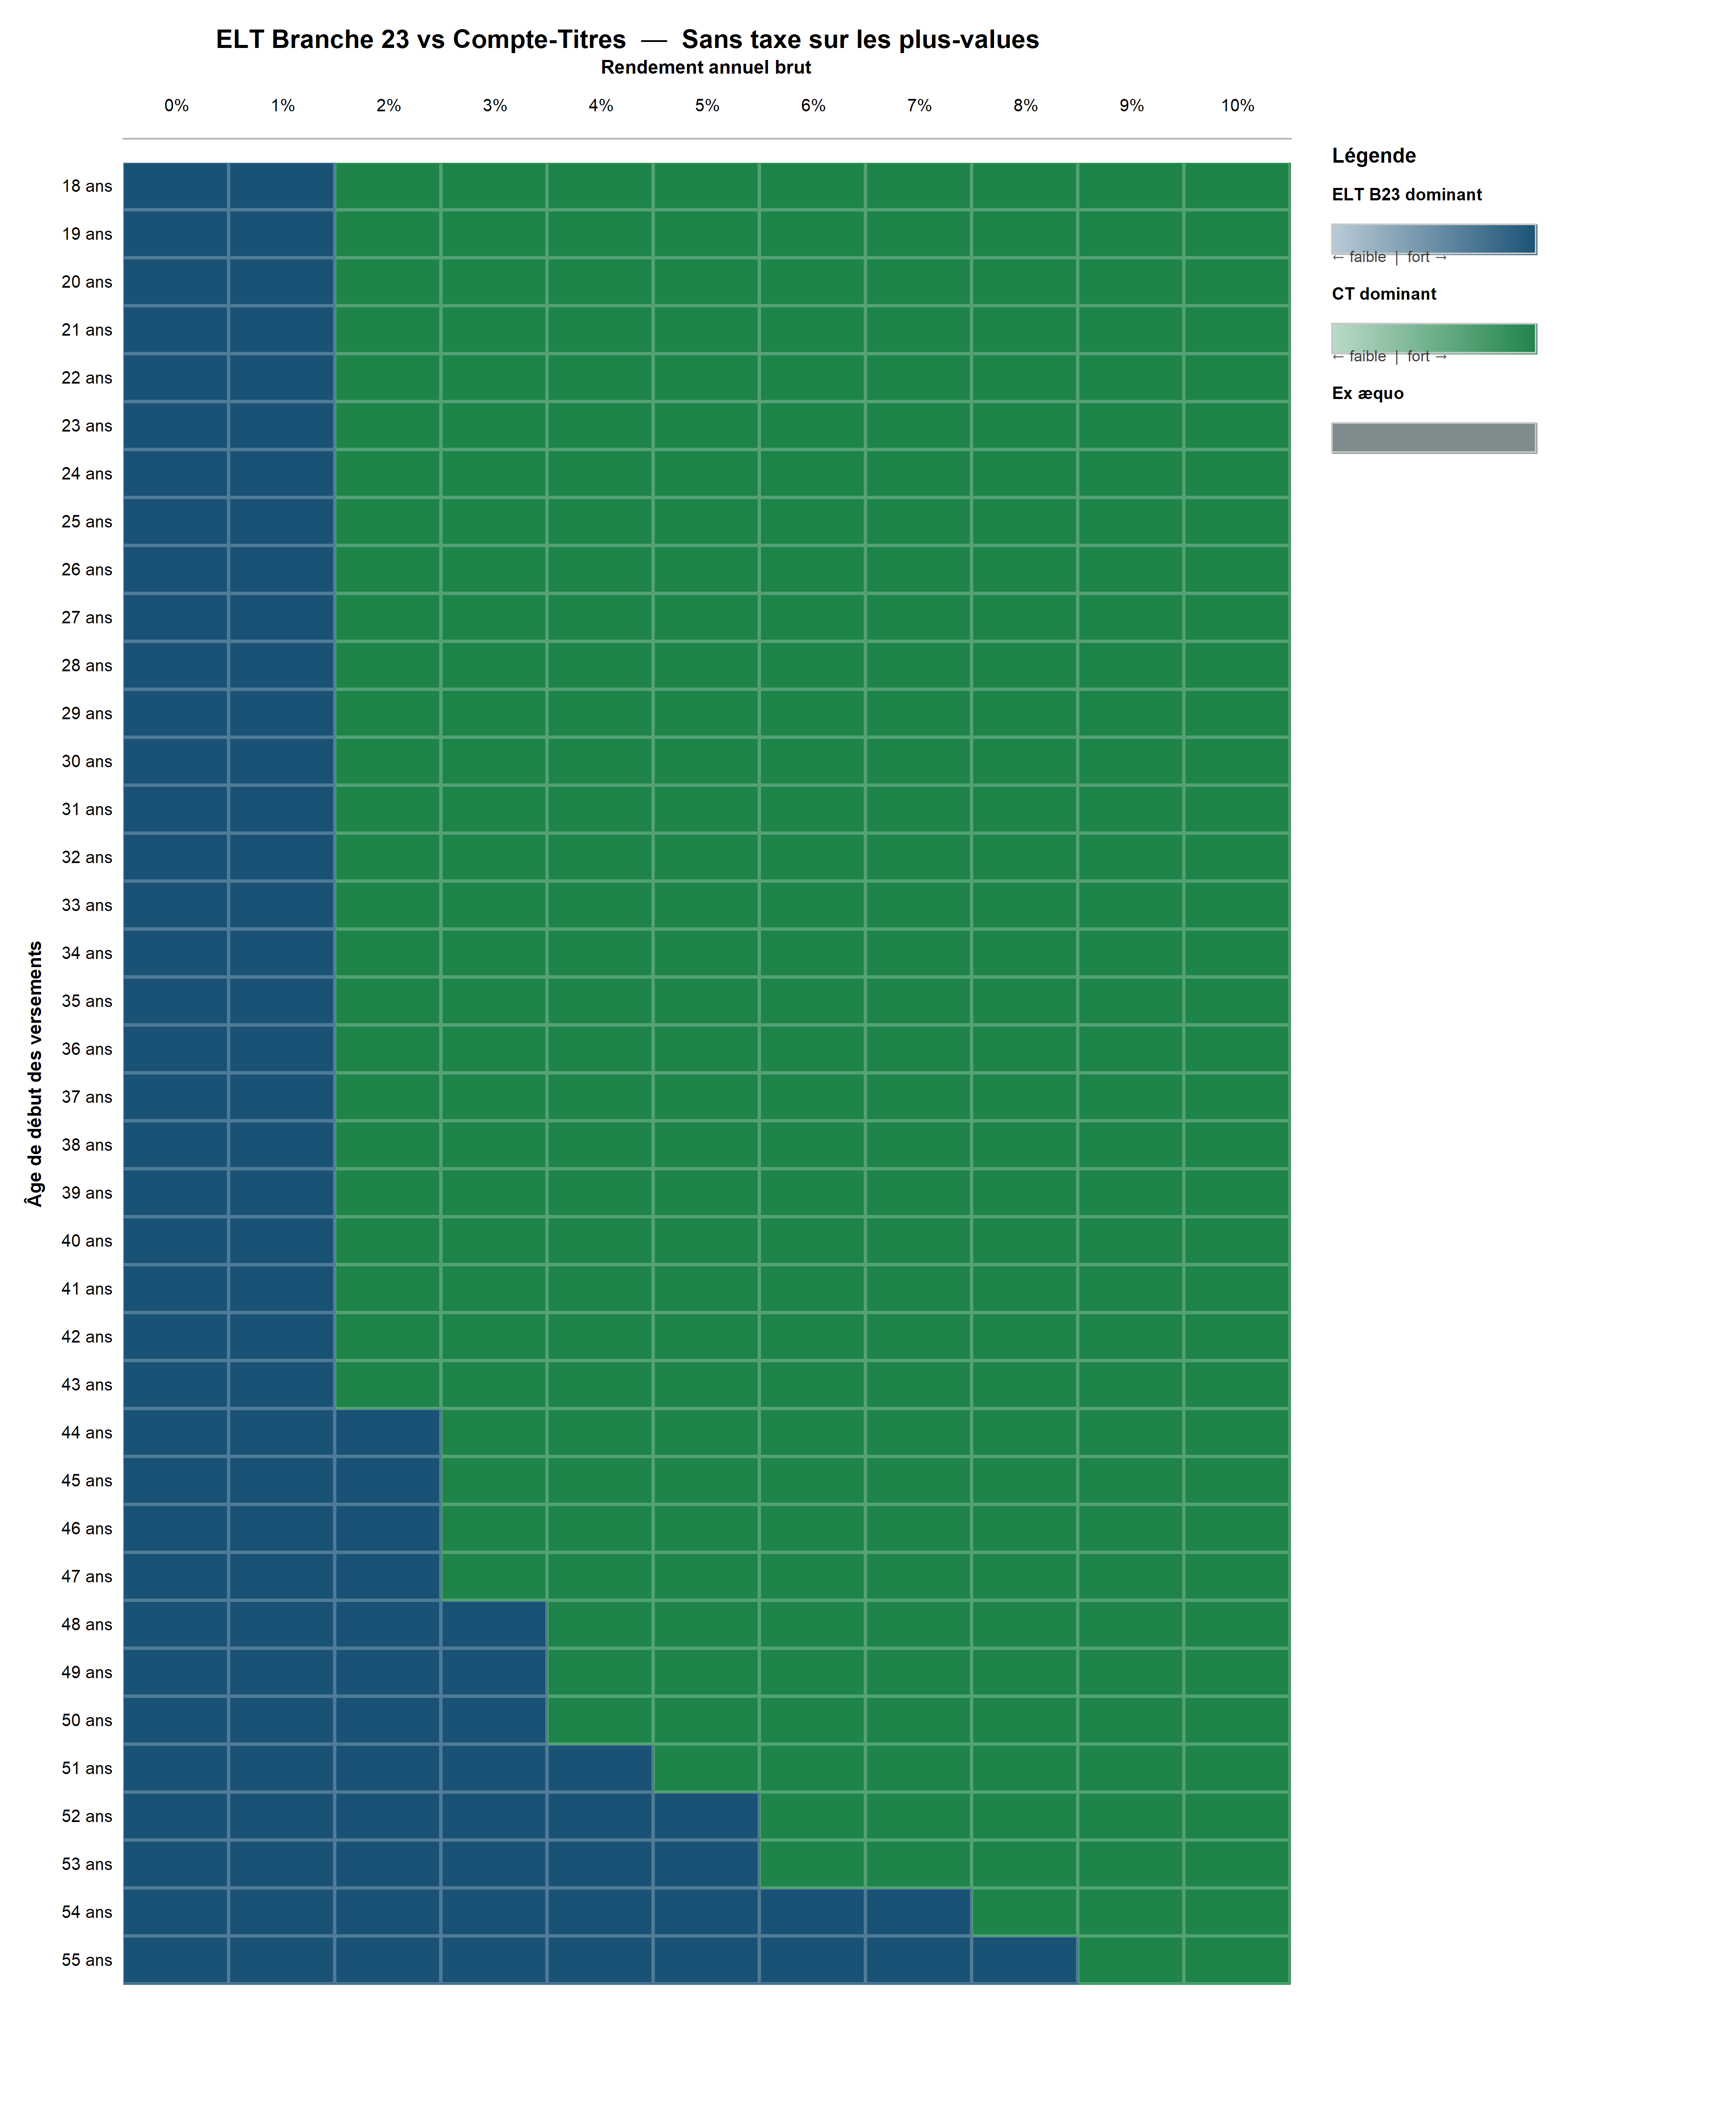
\includegraphics[width=0.485\linewidth]{media/elt_frais_reel_sans_taxe.png}%
\hfill%
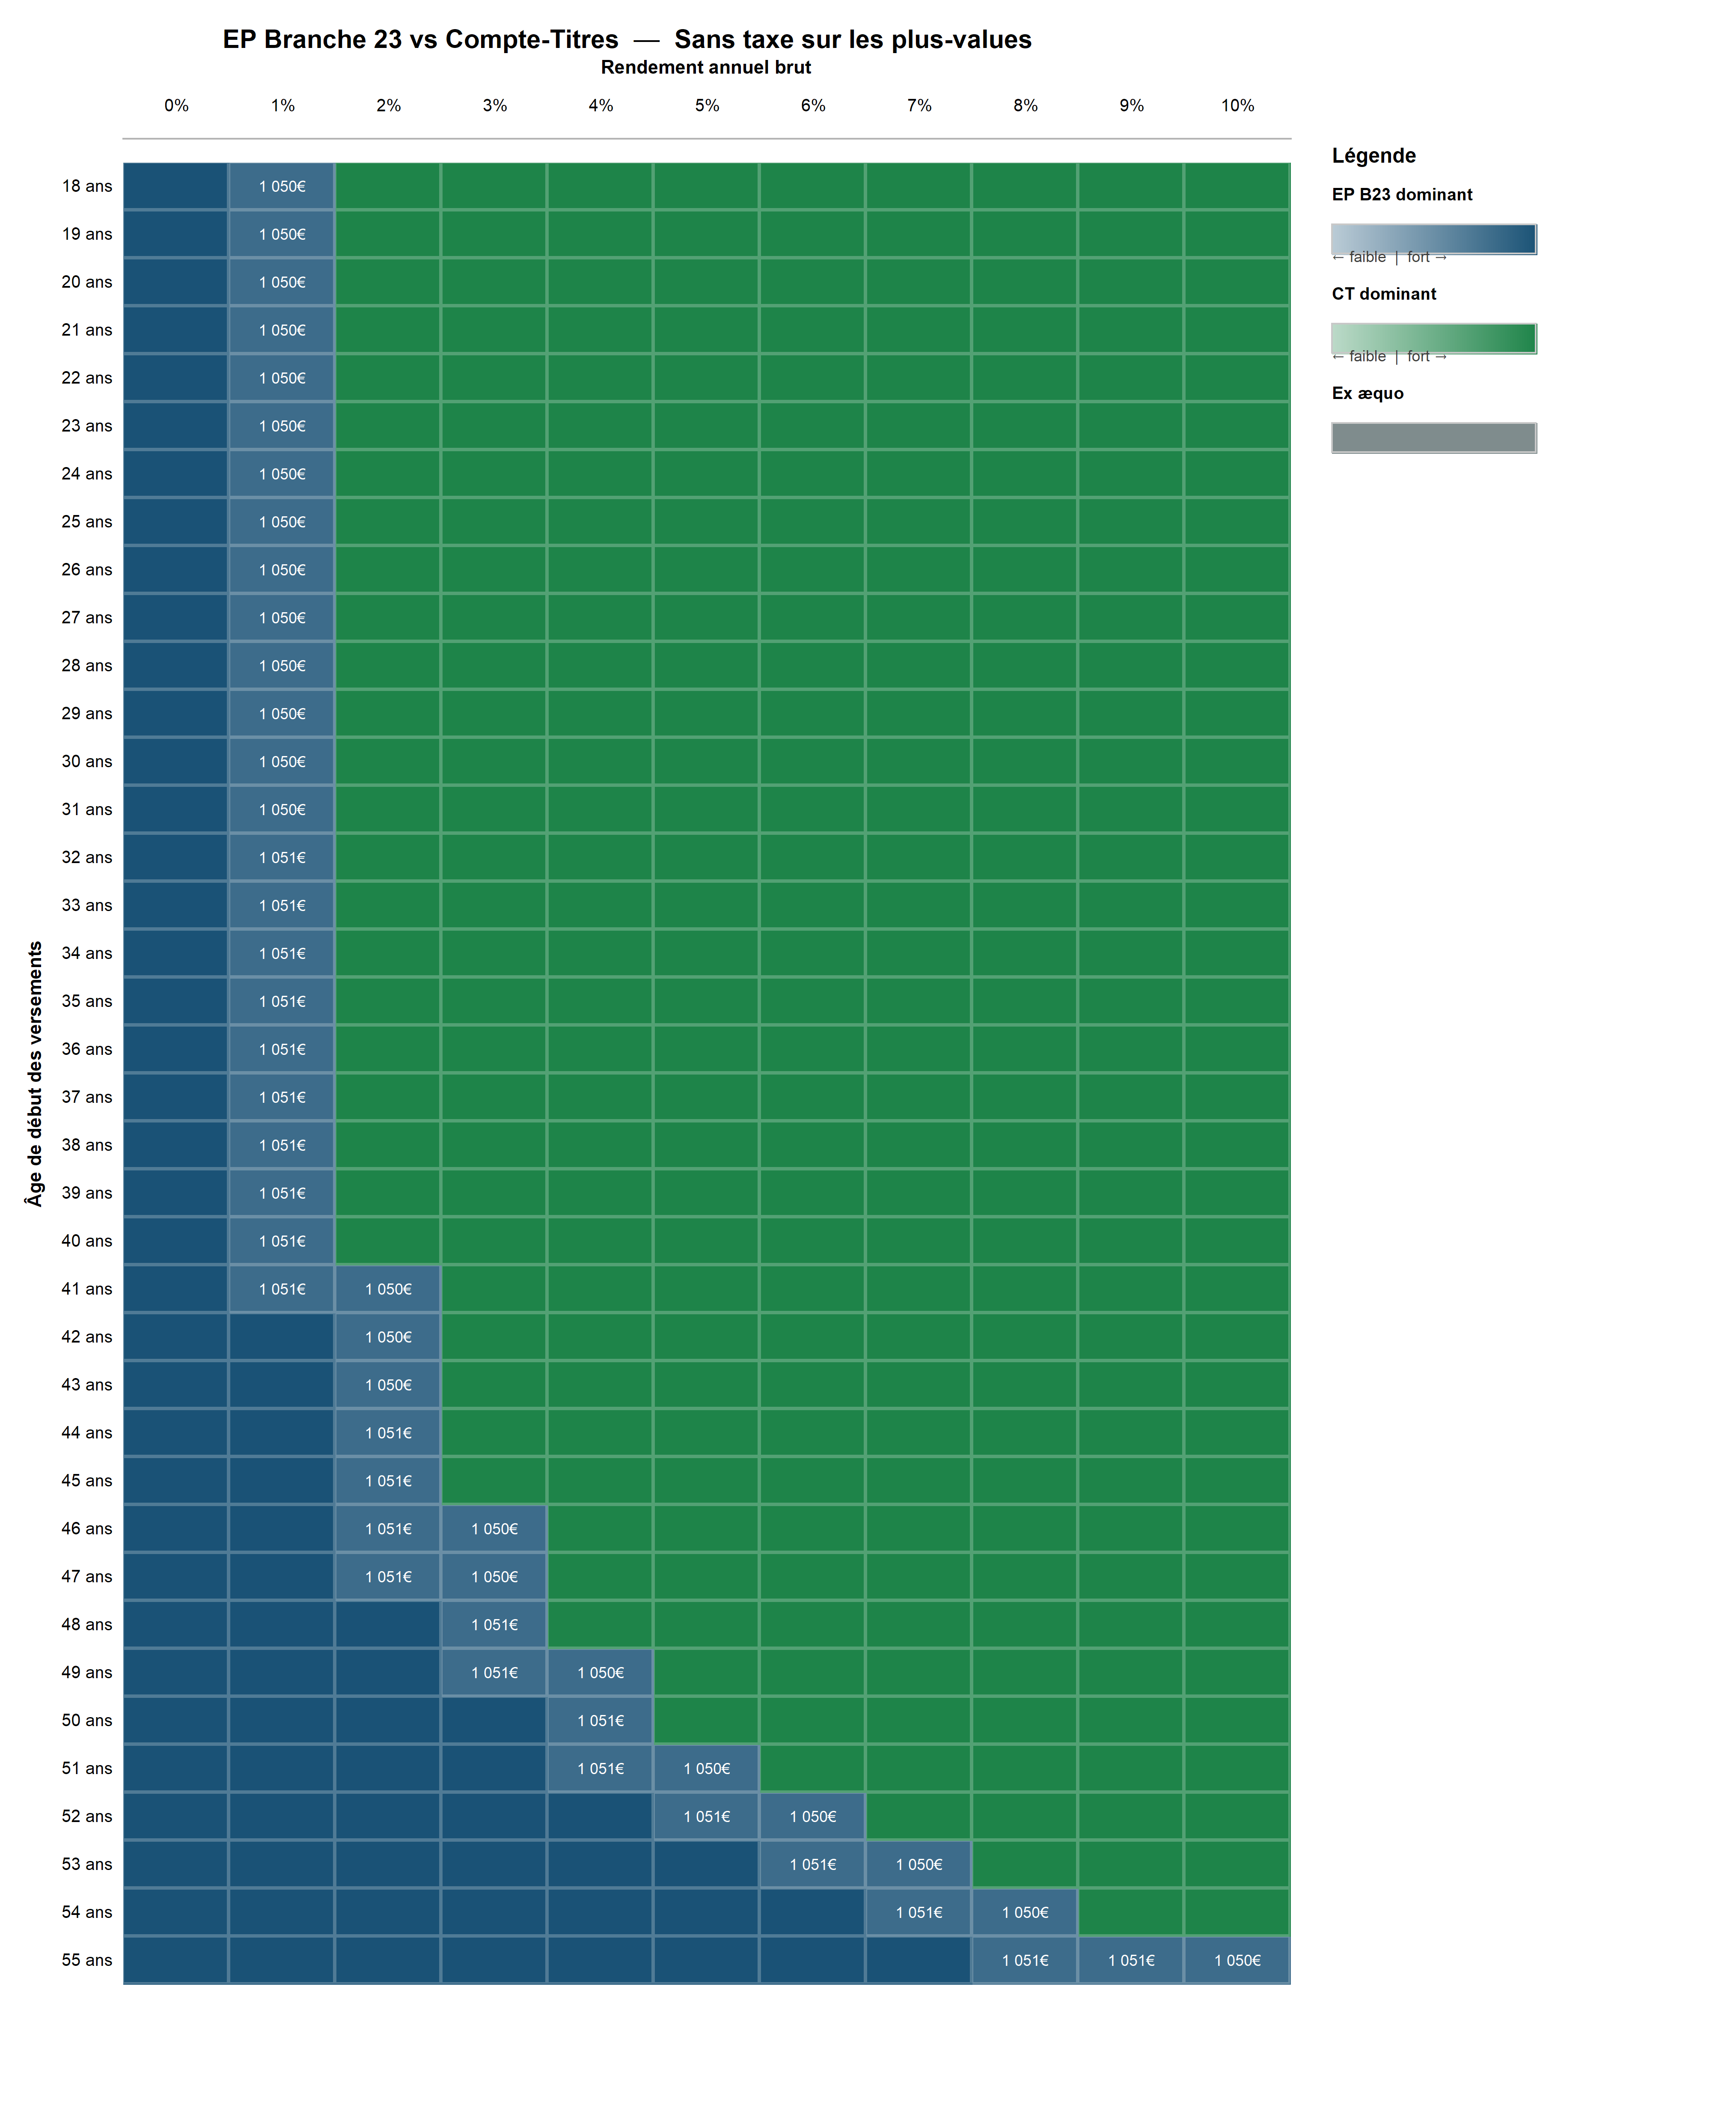
\includegraphics[width=0.485\linewidth]{media/ep_frais_reel_sans_taxe.png}
\par\vspace{1pt}
{\centering\scriptsize
  ELT vs CT (gauche) \quad EP vs CT (droite) \quad Scénario~B (frais réalistes), sans taxe PV\par
  \textcolor{b23color}{\rule{8pt}{6pt}}~B23 dominante \quad
  \textcolor{ctcolor}{\rule{8pt}{6pt}}~CT dominant \quad
  Intensité = force de dominance\par}

\vspace{5pt}

\textbf{Scénario~B --- frais réalistes (cas central)}

Le CT domine sur la grande majorité des configurations. La B23
ne s'impose qu'aux rendements faibles et horizons courts, où les
économies fiscales pèsent proportionnellement plus lourd que les
intérêts composés pas encore accumulés. \textbf{La taxe PV de~2026
érode le CT mais ne renverse pas cette hiérarchie}~: les frais de la B23
absorbent l'avantage fiscal, quelle que soit la réforme.

\vspace{4pt}

\textbf{Scénario~A --- frais nuls (effet fiscal pur)}

Sans frais, la B23 domine presque partout grâce à ses réductions
d'impôt. Ajoutez la taxe PV~: la B23 devient dominante sur la
quasi-totalité de la grille. C'est \textbf{l'effet fiscal à l'état pur}.

\vspace{4pt}

\textbf{Scénario~C --- frais égalisés}

Quand on supprime l'avantage tarifaire du CT, ses zones de dominance se
réduisent fortement. Il reste avantageux à rendement élevé et horizon
long~: ses frais sont prélevés \textit{en dehors} de la réserve,
contrairement à la B23 où ils sont déduits \textit{sur} le capital.

\vspace{4pt}

\textbf{Spécificité de l'EP~:} des seuils de croisement apparaissent
autour de \textbf{1\,050\,€/an}, correspondant au palier de réduction
d'impôt (30\,\% puis 25\,\%).

\vspace{4pt}

\begin{tcolorbox}[highlightbox]
\small
\textbf{Ce que le contenu grand public ne dit pas~:} à rendement
identique, \textbf{les frais récurrents} de la B23 pèsent
davantage que la fiscalité à la sortie. La taxe PV de~2026 n'invalide
pas le compte-titres dans le scénario réaliste. Ce sont les frais, plus
que le régime fiscal, qui déterminent la hiérarchie.
\end{tcolorbox}

\end{tcolorbox}
\end{minipage}

\end{document}
\small

\begin{tcolorbox}[highlightbox]
\small\centering
\textbf{Question de recherche~:}\\[3pt]
En 2026, en Belgique, dans une demarche d'investissement personnel
visant la constitution d'un capital retraite, lequel de
l'epargne-pension (EP), de l'epargne a long terme (ELT) ou du
compte-titres (CT) offre le \textbf{capital final net le plus eleve
a 65~ans}~? Dans quelle mesure la taxe sur les plus-values de~2026
modifie-t-elle cette hierarchie~?
\end{tcolorbox}

\vspace{5pt}

\begin{enumerate}[leftmargin=*, label=\textcolor{darkblue}{\bfseries\arabic*.}, itemsep=5pt]

  \item \textbf{Comparer} les trois vehicules sur un critere unique~:
    le \textbf{Capital Final Net (CFN)} a~65~ans, a hypotheses
    strictement identiques~: meme rendement brut, meme versement
    annuel, meme horizon.

  \item \textbf{Explorer} un large espace de parametres~:
    38~ages de debut (18 a 55~ans), 11~niveaux de rendement brut
    (0 a 10\,\%) et la plage complete de versements annuels
    de~1\,\texteuro{} jusqu'au plafond legal.

  \item \textbf{Mesurer l'impact de la reforme fiscale de~2026}~:
    la nouvelle taxe belge de~10\,\% sur les plus-values mobilieres,
    en vigueur depuis le 1\textsuperscript{er}~janvier~2026,
    modifie structurellement l'arbitrage entre vehicules.

  \item \textbf{Fournir un outil de lecture}~: les heatmaps
    produites identifient, pour chaque profil (age, rendement,
    versement), l'instrument dominant et les seuils de croisement.

\end{enumerate}

\end{tcolorbox}
\end{minipage}%
\hspace{10pt}%
\begin{minipage}[t]{\boxw}
\begin{tcolorbox}[posterbox, title=Pertinence du th\`eme]
\small

\begin{itemize}[leftmargin=*, label=\textcolor{darkblue}{\textbullet}, itemsep=8pt]

  \item \textbf{Reforme fiscale majeure de~2026~:} la Belgique
    introduit un impot de~10\,\% sur les plus-values mobilieres
    des particuliers, rompant avec l'absence historique de taxation.
    Les contrats d'epargne-pension et d'epargne a long terme sont
    explicitement exclus, creant une \textbf{asymetrie structurelle
    inedite} dans la comparaison des vehicules d'investissement.

  \item \textbf{Essor des neocourtiers et des ETF~:} le developpement
    de plateformes a frais reduits (Trade Republic, etc.) et la
    popularisation des ETF indiciels conduisent un nombre croissant
    de Belges a investir directement en compte-titres, en dehors de
    toute enveloppe institutionnelle, popularisant l'investissement
    passif comme alternative aux produits d'assurance-vie.

  \item \textbf{Comparaisons courantes biaisees~:} les analyses
    disponibles dans les medias attribuent frequemment des rendements
    differents selon le vehicule, invalidant leurs conclusions.
    Elles refletent l'hypothese retenue plutot que les
    caracteristiques intrinseques de chaque vehicule. Une comparaison
    a \textbf{rendement identique} s'impose.

  \item \textbf{Question d'actualite sans reponse systematique~:}
    l'arbitrage entre enveloppes fiscales et investissement direct
    est regulierement souleve sans jamais faire l'objet d'une analyse
    rigoureuse a hypotheses comparables couvrant l'ensemble de
    l'espace des parametres.

\end{itemize}

\end{tcolorbox}
\end{minipage}

\vspace{10pt}

% ==== LIGNE 2 ====
\noindent
\begin{minipage}[t]{\boxw}
\begin{tcolorbox}[posterbox, title=M\'ethodes mobilis\'ees]
\small

\textbf{Simulation deterministe}

Pour chaque combinaison de parametres, la trajectoire complete de
chaque vehicule est reconstituee jusqu'a~65~ans en appliquant
strictement les regles fiscales et tarifaires en vigueur.

\smallskip

\textbf{5\,016 combinaisons~: $38 \times 11 \times 4 \times 3$}, chacune
parcourant la plage de versements de~1\,\texteuro{} au plafond legal.

\vspace{5pt}

\textbf{Trois scenarios de frais}

\smallskip

\begin{tabular}{>{\bfseries\small}c >{\small}p{0.83\linewidth}}
  A & \textit{Sans frais} des deux cotes~: isole l'effet fiscal pur \\[2pt]
  B & \textit{Frais realistes}~: CT~=~0\,\%~;
      B23~=~2,83\,\% entree + 2,34\,\% gestion \\[2pt]
  C & \textit{Frais majores}~: CT calque sur les frais de B23
      (egalisation) \\
\end{tabular}

\vspace{5pt}

\textbf{Le Capital Final Net (CFN) --- critere unique}

\begin{tcolorbox}[inlinebox]
\small
Le CFN integre, ramenes a la meme date (65~ans) par capitalisation
au \textbf{taux OLO belge net de precompte (30\,\%)} (courbe BNB du
30~avril~2026)~: (1)~le capital net de taxe anticipative (B23) ou de
taxe sur les plus-values (CT)~; (2)~les economies fiscales annuelles
de la B23 capitalisees~; (3)~les couts capitalises a meme date.
\begin{equation*}
  \text{CFN} = C_N^{\text{net}}
  \;\pm\; \textstyle\sum\nolimits_t
    \text{Flux}_t \cdot (1+r_{\text{OLO}})^{n-t}
\end{equation*}
\end{tcolorbox}

\vspace{5pt}

\textbf{Heatmaps 2D} --- axe~X~: rendement brut (0--10\,\%)~;
axe~Y~: age de debut (18--55~ans). La couleur indique le vehicule
dominant et son intensite la force de la dominance. Les seuils de
croisement ($v^*$) sont annotes dans les cellules concernees.

\smallskip

\textbf{Validation}~: reproduction independante dans Excel (ligne par
ligne) et tests automatises de non-regression.

\end{tcolorbox}
\end{minipage}%
\hspace{10pt}%
\begin{minipage}[t]{\boxw}
\begin{tcolorbox}[posterbox, title=R\'esultats obtenus]
\small

\noindent
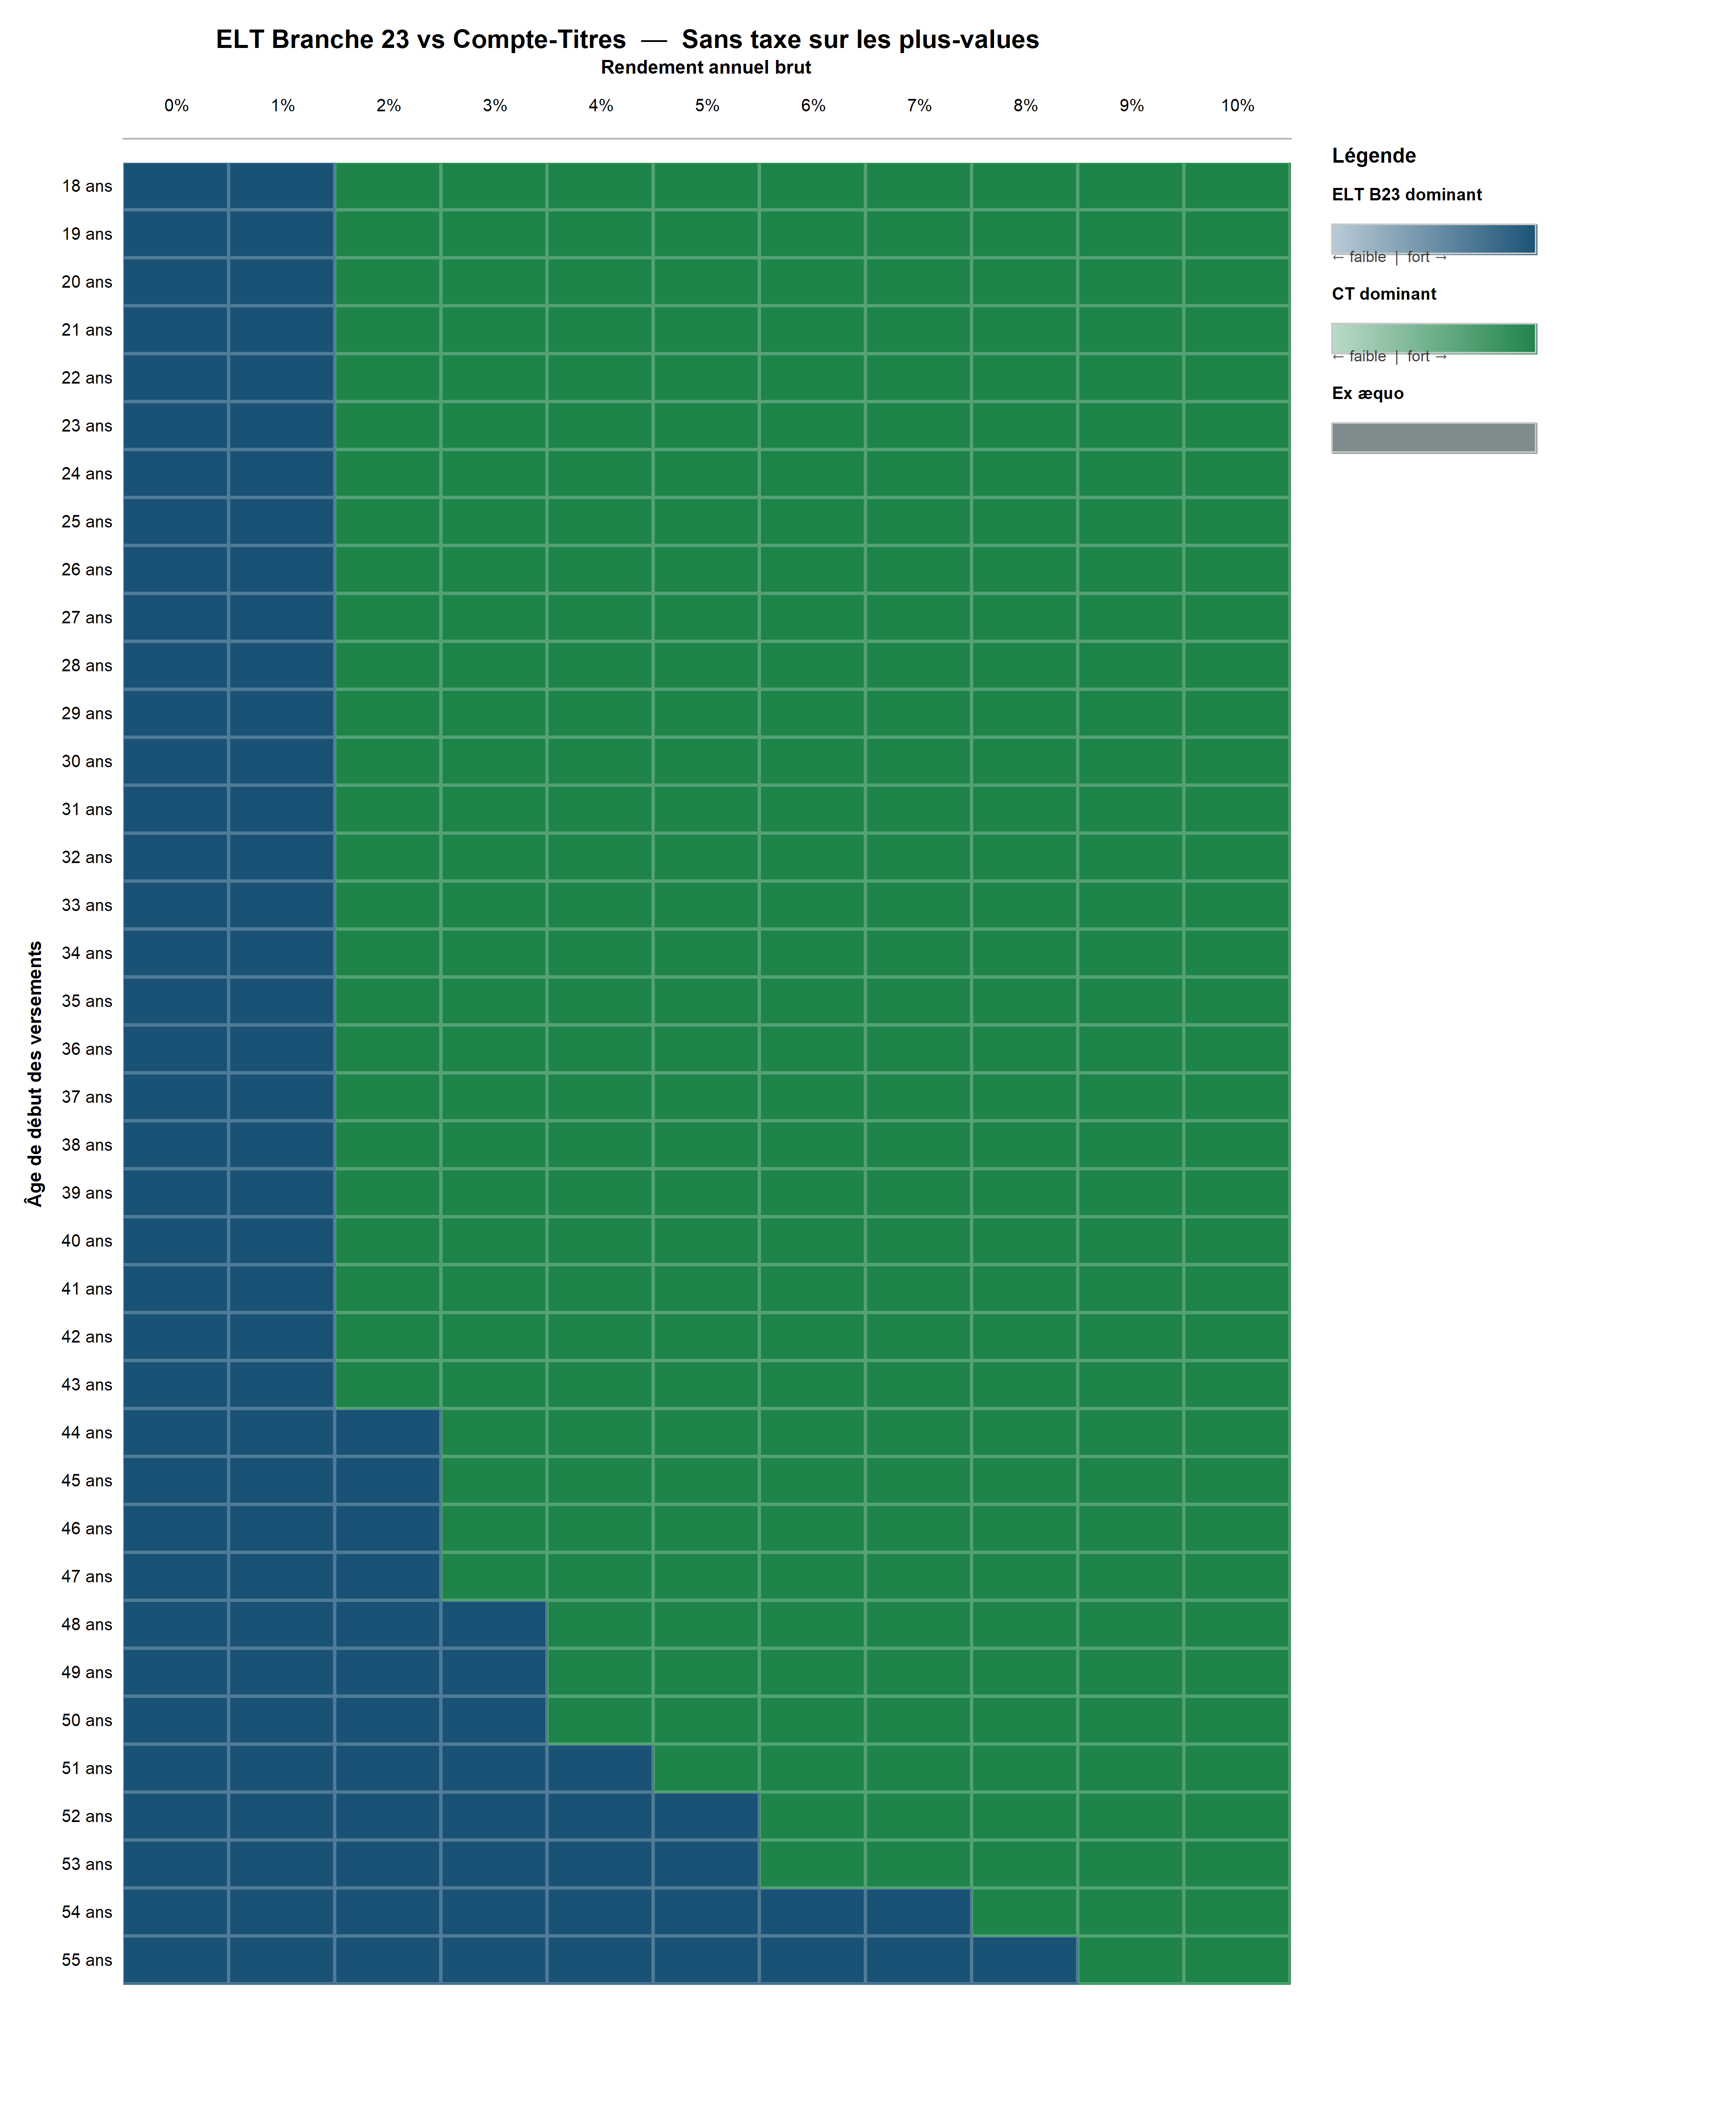
\includegraphics[width=0.485\linewidth]{media/elt_frais_reel_sans_taxe.png}%
\hfill%
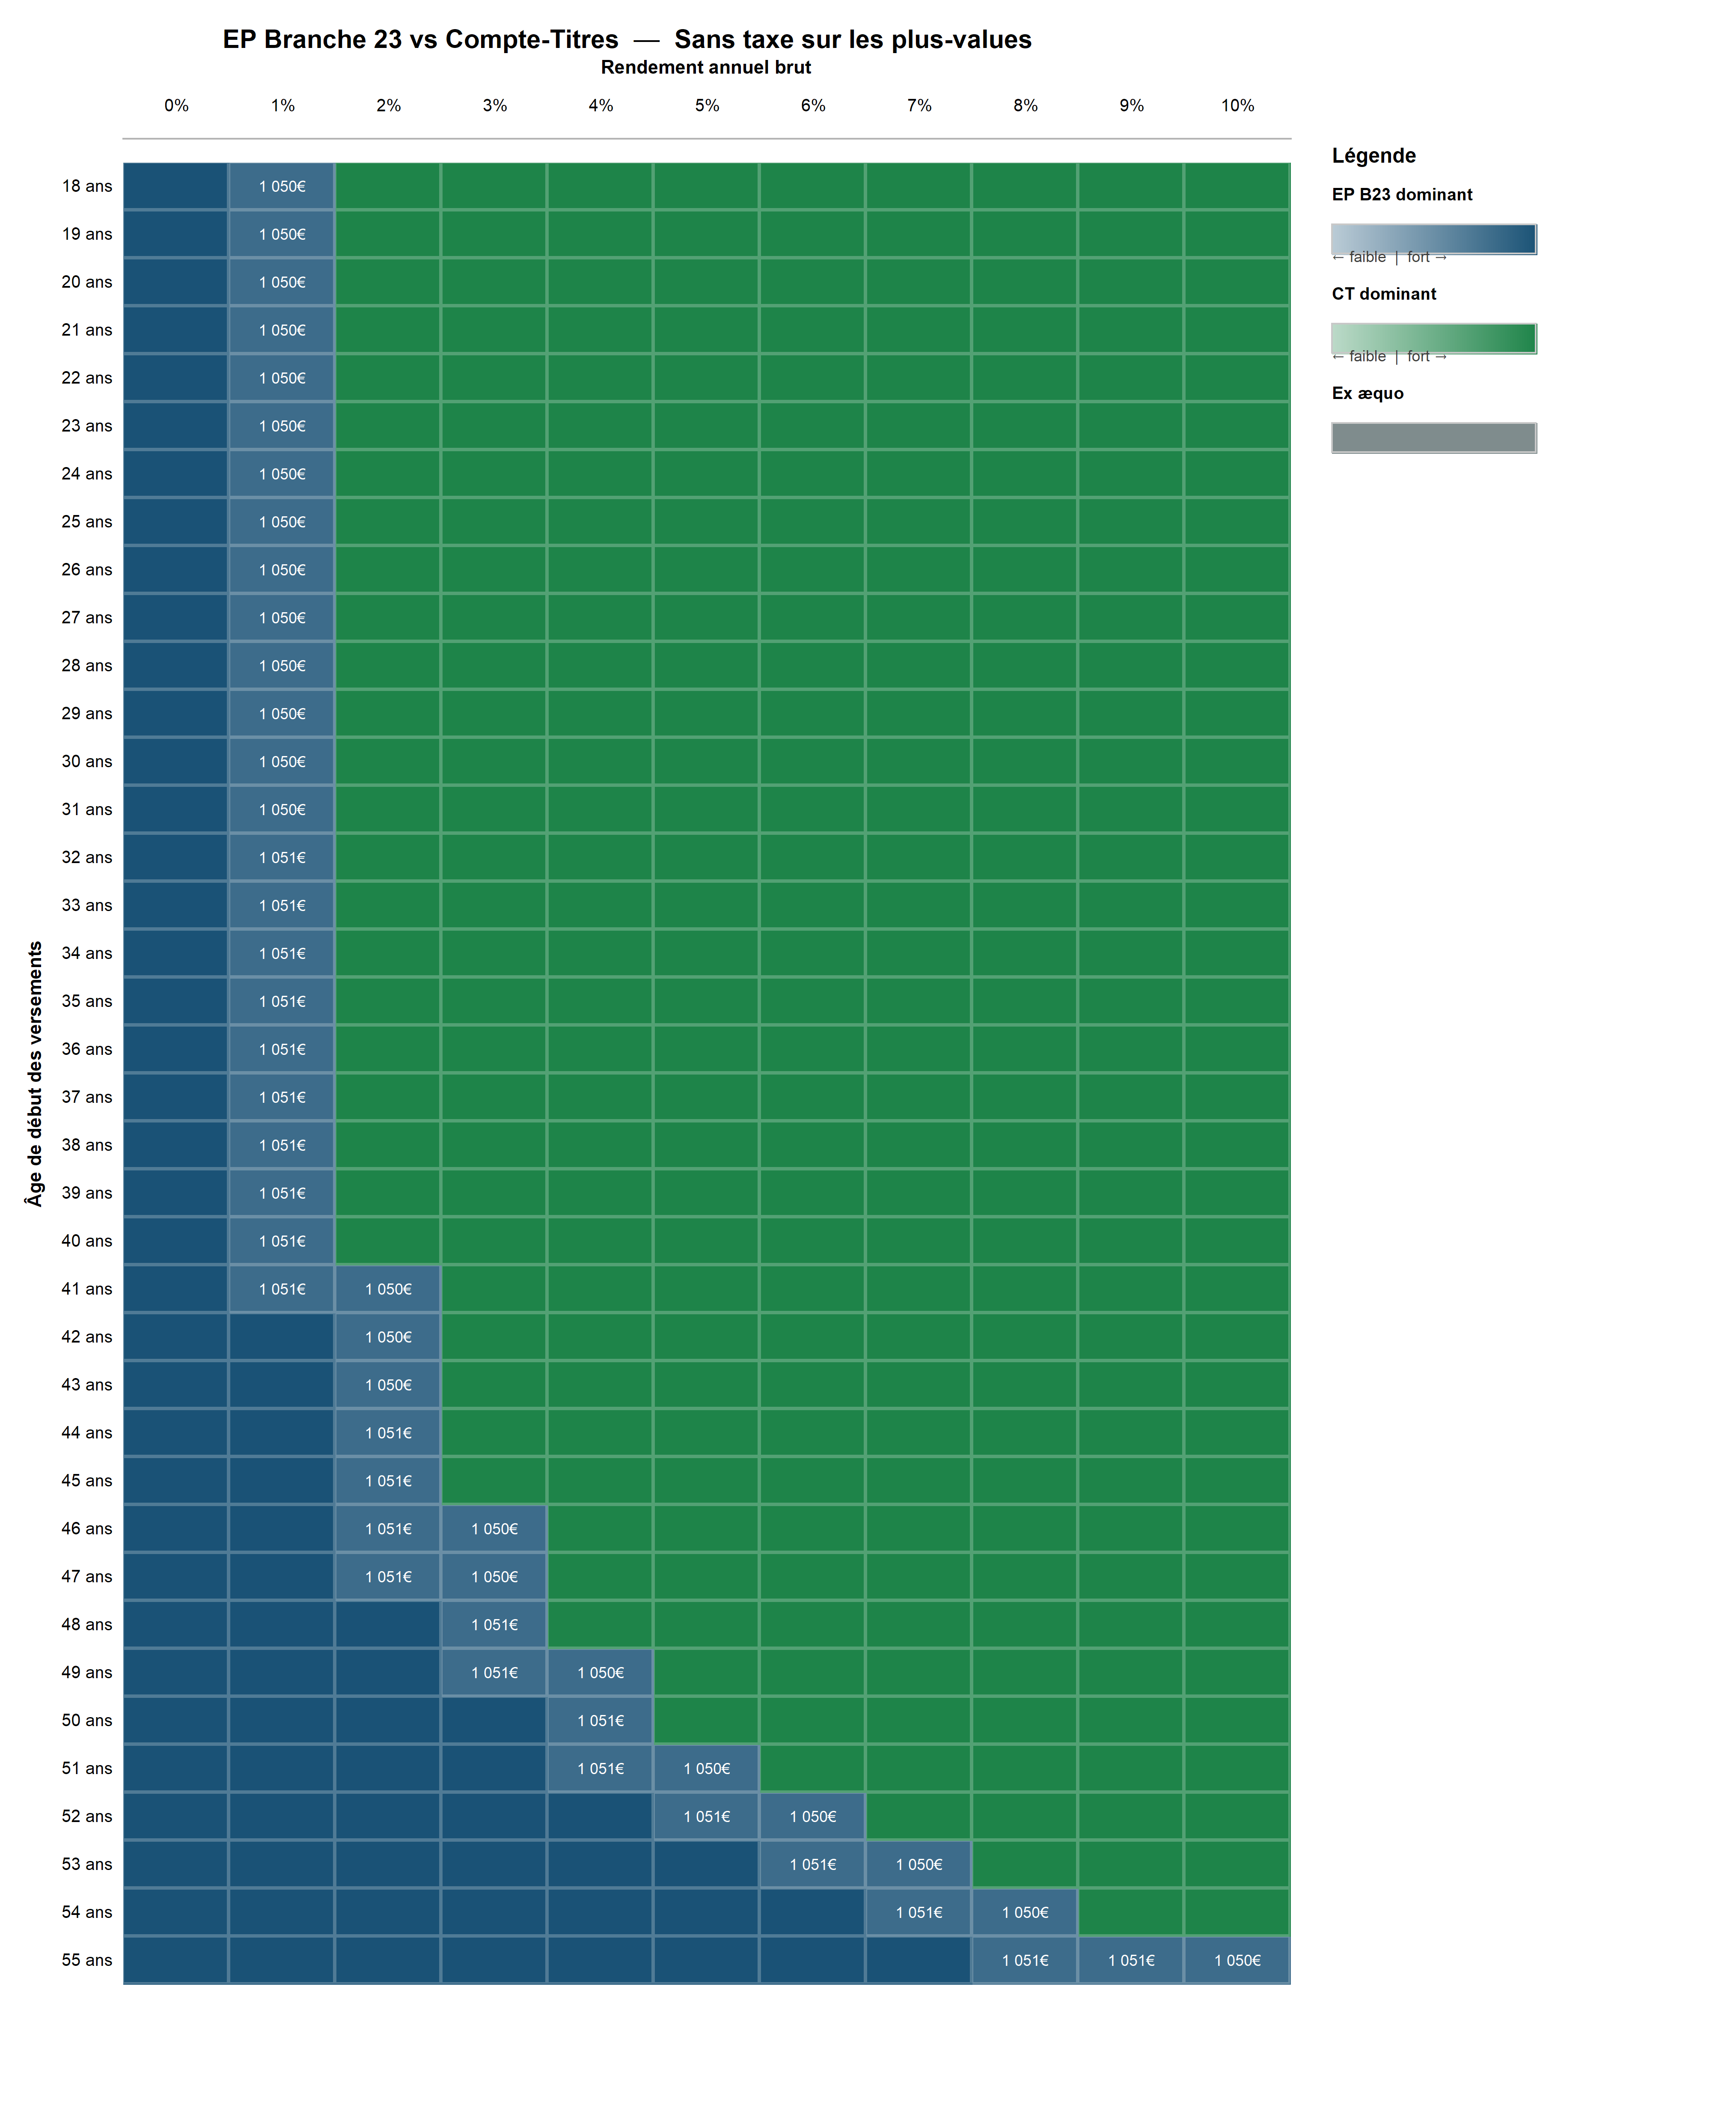
\includegraphics[width=0.485\linewidth]{media/ep_frais_reel_sans_taxe.png}
\par\vspace{1pt}
{\centering\scriptsize
  \textcolor{b23color}{\textbf{Bleu}}~= B23 dominante\enspace
  \textcolor{ctcolor}{\textbf{Vert}}~= CT dominant\enspace
  Intensite~= force\par}

\vspace{5pt}

\begin{itemize}[leftmargin=*, label=\textcolor{darkblue}{\textbullet}, itemsep=4pt]

  \item \textbf{Aucun vehicule universellement superieur}~: la
    hierarchie est sensible a l'age de debut, au rendement et
    surtout a la structure de frais.

  \item \textbf{Scenario realiste (B)~:} le \textbf{CT domine} sur
    la grande majorite des configurations. La branche~23 l'emporte
    uniquement aux rendements faibles ($\leq$\,3--4\,\%) et aux
    horizons courts.

  \item \textbf{Egalisation des frais (C)~:} les zones CT se
    reduisent fortement. \textbf{Les frais recurrents sont
    determinants}, davantage que la fiscalite a la sortie.

  \item \textbf{Taxe PV 2026~:} erode la rentabilite du CT sans
    renverser les resultats dans le scenario realiste. Son effet ne
    devient visible qu'en l'absence d'ecart tarifaire.

  \item \textbf{Epargne-pension~:} seuils de croisement autour de
    \textbf{1\,050\,\texteuro{}/an} (palier de reduction d'impot~:
    30\,\% en dessous, 25\,\% au-dessus).

\end{itemize}

\vspace{4pt}

\begin{tcolorbox}[highlightbox]
\small\centering
\textbf{Enseignement principal~:} les \textbf{frais recurrents}
pesent bien plus lourd que la fiscalite a la sortie sur le long
terme. La reforme de~2026 ne remet pas a elle seule en cause la
pertinence du CT pour un investisseur de long terme en ETF accumulant.
\end{tcolorbox}

\end{tcolorbox}
\end{minipage}

\end{document}